
\chapter{Enhancing the Creation of Mapping Rules}
\label{chapter:creation}

The mappings used for constructing knowledge graphs can be created in different ways. As they are formatted as text documents, they can be directly written in any text editor. However, the verbosity of some languages, the increased cognitive load required~\parencite{junior2018mental} and the need of following a specific syntax has fostered the development of user-friendly tools and serializations to ease the mapping writing process. This chapter introduces two alternative solutions for easing the construction of mappings for different potential users, (i) a spreadsheet-based approach to write the mapping rules (\cref{sec:chp5_mapeathor}), and (ii) a user-friendly mapping syntax updated with the latest needs in knowledge graph construction (\cref{sec:chp5_yarrrml_star}).

\section{Mapping rules in spreadsheets: Mapeathor}
\label{sec:chp5_mapeathor}

Since mapping languages started to be used more broadly, there have been multiple approaches for the development of editors to ease their specification. Some of them enable editing through graphical visualization~\citep{heyvaert2016rmleditor,sicilia2017map}, while others provide a writing environment (e.g. the Protégé extension OntopPro~\ana{ref}). These editors are language-oriented, as they help to create mappings in a specific language. However, use cases require different features and implementations, and as a result, several different mapping languages are used currently. Moreover, graphical interfaces may hinder the mapping management and creation when a large number of mapping rules is required. 

%Moreover, when managing large amounts of mapping rules, graphical interfaces become cumbersome. %With our approach we aim at easing the writing process using a common tool such as spreadsheets, as well as enabling the generation of mapping files in more than one mapping language.

%In our work we focus on facilitating the transformation rule specification using declarative mapping rules. 
This section presents a straightforward approach to create these mapping documents, leveraging the  specification of mapping rules in spreadsheets. These spreadsheets contain the essential elements of the mapping rules without any additional syntax element, and are later translated into one a mapping document. The purpose of this proposal is to increase the interoperability between these languages~\citep{corcho2020towards, iglesias2022devising} as well as to ease the creation process. To perform the mapping rules translation we developed Mapeathor~\citep{iglesias-molina_2023_5973906}, a tool able to parse the spreadsheets and generate the corresponding mappings in R2RML, RML and YARRRML. Following, we present the structure of the spreadsheet to write the mapping rules, the implementation and a evaluation with a user study to validate our approach.

\subsection{Spreadsheet design}
\label{sec:chp5_spreadsheet_design}

%The rules required to generate a knowledge graph can be specified in multiple languages. The language is chosen by the user depending on the specific use case. However, the rules themselves are equivalent across languages, so they can be written in a language-independent way, in this case, we chose a spreadsheet for rule specification. 

In this section we present the design of the spreadsheet template to write the mapping rules. 
These mapping rules are specified in the spreadsheets following a provided structure to only write the essential information. Thus, this approach prevents the user from learning the syntax peculiarities of each languages (e.g. keywords, semicolons, brackets, etc.).
This design is devised to represent the rules in a compact and understandable manner, using a format widely used by the scientific community (i.e. Google spreadsheets, MS Excel). 
Using these spreadsheets along with their corresponding editors allow users to leverage their native advantages.

The mapping rules are specified in the spreadsheet across five different sheets, which are described below: \textit{Prefix sheet}, \textit{Source sheet}, \textit{Subject sheet}, \textit{Predicate\_Object sheet} and \textit{Function sheet}. We illustrate this section with a running example to describe in detail the expressiveness capabilities of each spreadsheet. This example uses the data represented in the CSV file \texttt{people.csv}(\cref{lst:chp5_mapeathor_input_people}) and the JSON file \texttt{sport.json} (\cref{lst:chp5_mapeathor_input_sport}). 

\begin{minipage}{0.48\linewidth}
\begin{captionedlisting}{lst:chp5_mapeathor_input_people}{ Contents of \texttt{people.csv}.}
\centering
\begin{tabular}{c}
%\hspace{1em}
{
\begin{lstlisting}[basicstyle=\ttfamily\small,label={list:example1},columns=flexible]
id , name  , birthdate , sport_id
1  , Emily , 08/02/90  , 2
2  , Jonah , 18/11/75  , 2
\end{lstlisting}
}
\end{tabular}
\end{captionedlisting}
\end{minipage}
\,\,\,\,\hfill
\begin{minipage}{0.52\linewidth}
\begin{captionedlisting}{lst:chp5_mapeathor_input_sport}{Contents of \texttt{sport.csv}.}
\centering
\begin{tabular}{c}
\hspace{1.5em}
{
\begin{lstlisting}[basicstyle=\ttfamily\small,label={list:example1},columns=flexible]
[ {
   "id": 1,
   "sport": " Ice Skating"
 },{
   "id": 2,
   "sport": " Rugby"
 } ]
\end{lstlisting}
}
\end{tabular}
\end{captionedlisting}
\end{minipage}


\subsubsection{Prefix sheet} 
This sheet contains the namespaces and corresponding prefixes used in the creation of the transformation rules. 
It is composed of two columns: \texttt{Prefix} for the prefix and \texttt{URI} for the corresponding namespace. The base namespace can be specified writing ``@base" in the \texttt{Prefix} column. The namespaces used by the target mapping language are automatically added in the translation (e.g. \texttt{rr}\footnote{\url{http://www.w3.org/ns/r2rml\#}}, \texttt{rml}\footnote{\url{http://semweb.mmlab.be/ns/rml\#}}).
The example shown in \cref{tab:chp5_prefix_sheet} presents how three namespaces and the base namespace are written in this template. 

\begin{table}[h!]
\caption{Prefix sheet.}
\label{tab:chp5_prefix_sheet}
\centering
\begin{tabular}{c|c}
\midrule
\textbf{Prefix} & \textbf{URI}                                 \\ \midrule
@base           & http://example.com/                          \\
rdf             & http://www.w3.org/1999/02/22-rdf-syntax-ns\# \\
ex              & http://ex.com/                               \\ 
grel            & http://semweb.datasciencelab.be/ns/grel\#     \\
\midrule
\end{tabular}
\end{table}


\subsubsection{Subject sheet} 
This sheet defines how to generate the subjects and a corresponding identifier (\texttt{ID}) that groups the mapping rules per subject. It is organized in four columns: \texttt{ID}, \texttt{URI}, \texttt{Class} and \texttt{Graph}. \texttt{ID} contains a unique identifier for each subject's set of rules in order to relate to information on these rules in the remaining sheets.
\texttt{URI} defines the subject URI of the resources that are to be generated by the mapping. 
\texttt{Class} allows the assignation of the subject to a class with \texttt{rdf:type}. A subject may be type of one class, more than one or none at all. 
Finally, \texttt{Graph} is an optional column that enables the assignation of a named graph to the triples generated for a subject.

The example shown in \cref{tab:chp5_subject_sheet} presents how to write two subjects, each with a different identifier and URI for the instances. Within the \texttt{URI} field, what is written between ``\{" and ``\}" references a field in the source data. The instances of the subject with the \texttt{PERSON} ID are type of two classes, (\texttt{ex:Person} and \texttt{ex:Athlete}), while all the triples of the instances of the subject identified with the \texttt{SPORT} ID are assigned to a named graph (\texttt{ex:SportsGraph}). 


\begin{table}[h!]
\caption{Subject sheet.}
\label{tab:chp5_subject_sheet}
\centering
\begin{tabular}{c|c|c|c}
\midrule
\textbf{ID} & \textbf{URI} & \textbf{Class} & \textbf{Graph} \\ \midrule
PERSON & http://ex.com/Person/\{name\} & ex:Person &  \\
PERSON & http://ex.com/Person/\{name\} & ex:Athlete &  \\
SPORT & http://ex.com/Sport/\{sport\} & ex:Sport & ex:SportsGraph \\ \midrule
\end{tabular}
\end{table}

\ana{no class}


\subsubsection{Source sheet} 

This sheet describes the source input data for each set of rules, identified with the identifier previously created in the \textit{Subject sheet} (\texttt{ID}). The information is organized in three columns: \texttt{ID}, \texttt{Feature} and \texttt{Value}. 
\texttt{ID} makes reference to the identifier that gathers the mapping rules in the sheets, which was introduced in the \textit{Subject sheet}. 
\texttt{Feature} declares the type of information provided in \texttt{Value}. The allowed keywords in this column are: \texttt{source} for the path and name of the file, \texttt{format} for the data source format, \texttt{iterator} for hierarchical data (e.g. JSON, XML), \texttt{table} for name of tables from Relational Data Bases (RDBs), \texttt{query} for SQL queries and \texttt{SQLVersion} for the version of SQL used. Each ID must have at least the \texttt{source} and \texttt{format} features specified, the rest of the features are optional. 
Then, in the \texttt{Value} column, the corresponding values of each \texttt{Feature} specified are written. 

\cref{tab:chp5_source_sheet} shows the data source description for the \texttt{PERSON} and \texttt{SPORT} IDs. The former corresponds to the CSV file shown in \cref{lst:chp5_mapeathor_input_people}, while the latter to the JSON file in \cref{lst:chp5_mapeathor_input_sport}, for which the iterator is also written (\texttt{\$.*}). 

\begin{table}[h!]
\caption{Source sheet.}
\label{tab:chp5_source_sheet}
\centering
\begin{tabular}{c|c|c}
\midrule
\textbf{ID} & \textbf{Feature} & \textbf{Value}              \\ \midrule
PERSON    & source          & /home/user/data/people.csv  \\
PERSON    & format          & CSV                         \\
SPORT     & source          & /home/user/data/sports.json \\
SPORT     & format          & JSON                        \\  
SPORT     & iterator        & \$.*                    \\ \midrule
\end{tabular}
\end{table}

\subsubsection{Predicate\_Object sheet} 
This sheet enable users to specify how to generate the triples, that is, predicate-object pairs for the subjects defined in the \textit{Subject sheet}. This sheet contains up to 8 columns: \texttt{ID}, \texttt{Predicate}, \texttt{Object}, \texttt{DataType}, \texttt{Language}, \texttt{ReferenceID}, \texttt{InnerRef} and \texttt{OuterRef}.

The column \texttt{ID} indicates the set of rules which the triples belong to, that has been previously defined in the \textit{Subject} and \textit{Source sheets}.
The columns \texttt{Predicate} and \texttt{Object} specify the predicate and object of the triple respectively. 
The XSD datatype of \texttt{Object} is defined in \texttt{DataType}, and the language tag in \texttt{Language}. Both these columns are optional. 

When the object refers to a subject defined in another mapping rule, the rule is written as follows. 
There are three columns that allow the specification of the linking condition between the object of the current triple and the referenced subject. 
They specify which is the ID of the referred subject  (\texttt{ReferenceID}), and the ``join'' fields in the source data: (i) \texttt{InnerRef} for the field of the object of the current triple, and (ii) \texttt{OuterRef} for the field of the referred subject. These three fields can be blank when a regular triple is produced. 

\cref{tab:chp5_po_sheet} shows five predicate-object pairs created for both sets of rules (\texttt{PERSON} and \texttt{SPORT}. Three of these rules produce literals with datatypes and two additionally specify a language tag. The rule set identified as \texttt{PERSON} generates a link to the subject of the \texttt{SPORT} rule set using the predicate \texttt{ex:name}, and joining by equal values of the field \texttt{sport\_id} from \texttt{people.csv} and the field \texttt{id} from \texttt{sport.json}. This rule set also calls a function for generating the object for the predicate \texttt{ex:birthdate}, which is identified by being enclosed by ``$<>$".

\begin{table}[h!]
\caption{Predicate\_Object sheet.}
\label{tab:chp5_po_sheet}
\centering
\resizebox{\columnwidth}{!}{
\begin{tabular}{c|c|c|c|c|c|c|c}
\midrule
\textbf{ID} &\textbf{Predicate} & \textbf{Object}               & \textbf{DataType} & \textbf{Language} & \textbf{ReferenceID} & \textbf{InnerRef} & \textbf{OuterRef} \\ \midrule
PERSON & ex:name & \{name\} & string & en & & &  \\
PERSON & ex:birthdate & $<$Fun-date$>$ & & & & & \\
PERSON & ex:plays & & & & SPORT& sport\_id & id \\
SPORT & ex:name & \{sport\} & string & en & & & \\
SPORT & ex:code & \{id\} & integer & & & & \\ \midrule
\end{tabular}
}
\end{table}

\subsubsection{Function sheet} Some languages are able to process data transformation functions, which can be detailed in this sheet. Mapeathor implements the last release of the RML-FNML specification, that describes how to incorporate functions in RML mappings\footnote{\url{https://w3id.org/rml/fnml/spec}}. The functions are referred in the \textit{Predicate\_Object sheet} or in other function rows with the identifier specified in \texttt{FunctionID}. The column \texttt{Feature} is used to specify the type of information provided in \texttt{Value}. The features admitted in the \texttt{Feature} column are \texttt{executes} for the name of the function, and \texttt{returns} for the expected output type of the function. In addition, this column admits any number of function parameter names. Then, the value of the name of the function, return type and values of the parameters are written correspondingly in the \texttt{Value} column.

The example shown in \cref{tab:chp5_function_sheet} uses the function \texttt{grel:toDate}, to change the formatting of a date. It returns a date as output (\texttt{grel:dateOut}) and takes three parameters: the data field to be converted (\texttt{grel:valueParam1}), the input data format (\texttt{grel:valueParam2}) and the output data format (\texttt{grel:valueParam3}).

\begin{table}[h!]
\caption{Function sheet.}
\label{tab:chp5_function_sheet}
\centering
\begin{tabular}{c|c|c}
\midrule
\textbf{FunctionID} & \textbf{Feature} & \textbf{Value} \\ \midrule
$<$Fun-date$>$ & executes & grel:toDate \\  
$<$Fun-date$>$ & returns & grel:dateOut \\  
$<$Fun-date$>$ & grel:valueParam1 & \{birthdate\} \\
$<$Fun-date$>$ & grel:valueParam2 & dd/MM/yyyy \\
$<$Fun-date$>$ & grel:valueParam3 & yyyy-MM-dd \\
\midrule
\end{tabular}
\end{table}


\subsection{Mapeathor}
\label{sec:chp5_mapeathor_tool}

Mapeathor~\citep{iglesias-molina_2023_5973906} is a open-source implementation to generate mappings from the spreadsheets described in \cref{sec:chp5_spreadsheet_design}. It is able to process MS Excel and Google Spreadsheets, generating human-readable mappings in either R2RML, RML or YARRRML. 

\cref{alg:mapeathor} presents the procedure implemented by Mapeathor to translate an input spreadsheet into a formatted mapping document. First, the rules written in the spreadsheet template are extracted and stored in a JSON file. This step also validates that the spreadsheet follows correctly the template. The prefixes are then added to the output mapping document, along with other prefixes that are used nativetly in the target language (e.g. \texttt{r2rml}, \texttt{rml} \ana{prefijo rml}). Then, the rules are translated by grouping them into rulesets with the same \texttt{ID} expressed in the spreadsheet (see \ana{previous section with template and subject)}. The extracted rules are enriched with implicit information needed to write the mapping (e.g. to look for \textit{rr:TermTypes} and IRIs). Next, the subject, source and predicate-object pairs in each ruleset are translated. In the case of RML, the system also looks for referencing functions to translate them as well. Finally, the translated rules are written into a final file, which is returned as output. The mapping documents are written by the system in a human-readable manner. \ana{ojo que esto se parece a yatter } \ana{listing whatever } shows the output RML mapping that Mapeathor produces after processing the rules written in the spreadsheet shown in Tables \ref{tab:chp5_prefix_sheet}, \ref{tab:chp5_subject_sheet}, \ref{tab:chp5_source_sheet}, \ref{tab:chp5_po_sheet} and \ref{tab:chp5_function_sheet}. 


The source code of Mapeathor is openly available under Apache 2.0 license\footnote{\url{https://github.com/oeg-upm/mapeathor}}. It can be run as a CLI using the Pypi package\footnote{\url{https://pypi.org/project/mapeathor/}} or as an online service\footnote{\url{https://morph.oeg.fi.upm.es/demo/mapeathor}}, where a visual interface is provided. With each release, a new version in Pypi is created and a dedicated DOI archived in Zenodo~\citep{iglesias-molina_2023_5973906}. 


\begin{minipage}{0.95\linewidth}
\begin{algorithm}[H]
\SetAlgoLined
\KwResult{Mapping document in [R2]RML/YARRRML}
 $language \longleftarrow output\_language$\;
 $spreadsheet \longleftarrow input\_spreadsheet$\;
 $output\_m \longleftarrow \emptyset$\;
 $rules \longleftarrow extract\_rules(spreadsheet)$\;
 $output\_m.add(translate\_prefixes(rules))$\;
  
 \For{$ruleset \in rules$}{
    $rules.add(enrich\_ruleset(ruleset))$\;
    $output\_m.add(translate\_subject, language)$\;
    $output\_m.add(translate\_source, language)$\;
    $output\_m.add(translate\_predicate\_object, language)$\;
    \If{$language == RML$}{
        $output\_m.add(translate\_functions)$\;
        }
    }
 
 \Return{$validate(write\_m)$}\;
\caption{Mapeathor translation algorithm}
\label{alg:mapeathor}
\end{algorithm}
\end{minipage}

\begin{captionedlisting}{lst:chp5-1_rml-output}{RML mapping generated with Mapeathor with the spreadsheet shown in Tables \ref{tab:chp5_prefix_sheet}, \ref{tab:chp5_subject_sheet}, \ref{tab:chp5_source_sheet}, \ref{tab:chp5_po_sheet} and \ref{tab:chp5_function_sheet}. }
\centering
{\begin{lstlisting}[numbers=left,basicstyle=\ttfamily\small,columns=flexible]
@prefix rr: <http://www.w3.org/ns/r2rml#>.
@prefix xsd: <http://www.w3.org/2001/XMLSchema#>.
@prefix rml: <http://semweb.mmlab.be/ns/rml#>.
@prefix ql: <http://semweb.mmlab.be/ns/ql#>.
@prefix rdf: <http://www.w3.org/1999/02/22-rdf-syntax-ns#>.
@prefix ex: <http://ex.com/>.
@prefix grel: <http://semweb.datasciencelab.be/ns/grel#>.
@base <http://example.com/>.

<#PERSON>
    a rr:TriplesMap;
    rml:logicalSource [
    	rml:source "/home/user/data/people.csv";
    	rml:referenceFormulation ql:CSV;
    ];
    rr:subjectMap [
    	a rr:Subject ;
    	rr:termType rr:IRI ;
    	rr:template "http://ex.com/Person/{name}" ;
    	rr:class ex:Person ;
    	rr:class ex:Athlete ;
    ];
    rr:predicateObjectMap [
    	rr:predicateMap	[ rr:constant ex:name];
    	rr:objectMap	[ rml:reference "name"; 
                      rr:termType rr:Literal;  
                      rr:datatype xsd:string;  
                      rr:language "en" ]
    ];
    rr:predicateObjectMap [
    	rr:predicateMap	[ rr:constant ex:plays ];
    	rr:objectMap	[
    		rr:parentTriplesMap	<#SPORT>;
    		rr:joinCondition	[
    			rr:child	"sport_id";
    			rr:parent	"id";
    		];
    	];
    ];
    rr:predicateObjectMap [
      rr:predicateMap	[ rr:constant ex:birthdate] ;
      rr:objectMap	[
    	  rml:functionExecution <#Fun-date> ;
    	  rml:return grel:dateOut ;
    	];
    ]; .

<#SPORT>
    a rr:TriplesMap;
    rml:logicalSource [
    	rml:source "/home/user/data/sports.json";
    	rml:referenceFormulation ql:JSONPath;
        rml:iterator "$\dollar$.*";
    ];
    rr:subjectMap [
    	a rr:Subject ;
    	rr:termType rr:IRI ;
    	rr:template "http://ex.com/Sport/{sport}" ;
    	rr:class ex:Sport ;
    	rr:graphMap [ rr:constant "ex:SportsGraph" ] ;
    ];
    rr:predicateObjectMap [
    	rr:predicateMap	[ rr:constant ex:name];
    	rr:objectMap	[ rml:reference "sport";  
                      rr:termType rr:Literal;  
                      rr:datatype xsd:string;  
                      rr:language "en" ]
    ];
    rr:predicateObjectMap [
    	rr:predicateMap	[ rr:constant ex:code];
    	rr:objectMap	[ rml:reference "id";  
                      rr:termType rr:Literal;  
                      rr:datatype xsd:integer ]
    ]; .

<#Fun-date> a rml:FunctionExecution;
    rml:function grel:toDate ;
    rml:input [
      a rml:Input ;
      rml:parameter grel:valueParam1 ;
      rml:inputValueMap [ rml:reference "birthdate" ];
    ];
    rml:input [
      a rml:Input ;
      rml:parameter grel:valueParam2 ;
      rml:inputValueMap [ rr:constant "dd/MM/yyyy" ];
    ];
    rml:input [
      a rml:Input ;
      rml:parameter grel:valueParam3 ;
      rml:inputValueMap [ rr:constant "yyyy-MM-dd" ];
    ]; .
\end{lstlisting}}
\end{captionedlisting}

\subsection{Evaluation}
We evaluate the presented approach by performing a user study with two dimensions to test the usability of Mapeathor and check if the spreadsheet-based approach can improve the mapping writing process for users of different expertise. 

\begin{table}[t!]
\caption{Questionnaire for subjective assessment of the usability of the spreadsheet design and Mapeathor. }
\centering
\label{tab:chp5_sub_questionnaire}
\resizebox{\columnwidth}{!}
{\begin{tabular}{cl}
\multicolumn{2}{c}{\textbf{Questions}} \\ \midrule
1. & I think that I would like to use this tool frequently\\ \midrule
2. & I found the tool unnecessarily complex\\ \midrule
3. & I thought the spreadsheet template was easy to use\\ \midrule
4. & I think that I would need the support of a technical person to be able to use the spreadsheet template\\ \midrule
5. & I found the different facets in this spreadsheet template were well integrated\\ \midrule
6. & I thought there was too much inconsistency in this tool\\ \midrule
7. & I think that most people would learn how to write the spreadsheet template very quickly\\ \midrule
8. & I found the tool unmanageable to use\\ \midrule
9. & I felt very confident using the spreadsheet template\\ \midrule
10. & I needed to learn a lot of things before I could get going with this tool\\ \midrule
11. & Optional comments (feedback to improve) \\ \bottomrule
\end{tabular}}
\end{table}

\subsubsection{Methodology}
\label{sec:chp5_mapeathor_eval_method}

The evaluation is performed in two steps. We first carry out a \textit{subjective evaluation} in order to gather opinions and feedback about the spreadsheet template and usability of the tool in order to improve the user experience. We then perform a \textit{objective evaluation} to find out if our approach improves the mapping writing process w.r.t. writing directly the mapping in a target language (i.e. RML) and w.r.t. another mapping editor with a visual interface (i.e. RMLEditor). This section describes the methodology followed for the performed evaluations.

%\textit{motivación: qué queremos comprobar, que si facilita la creación de mapping rules para experts y no experts. Para eso llevamos a cabo dos evaluaciones con usuarios, subjectiva y objetiva. En la subjectiva usuarios que han probado el software cuentan su experiencia y opiniones. En la objetiva, cogemos a usuarios y los dividimos en 3 grupos, para que generen mappings con rml, rmleditor y mapeathor. Así vemos si 1) mapeathor mejora RML y si 2) funciona mejor que una herramienta visual. Describir background, que no hay bias porque se puso a gente que nos había utilizado esa tech antes. y resultados}


\noindent\textit{\textbf{Procedure}} The evaluation is comprised of two steps. The first step, correspondent to the \textit{subjective evaluation}, took place during the Knowledge Graph Construction Tutorial co-located with the 19th edition of the Extended Semantic Web Conference (2022)\footnote{\url{https://kg-construct.github.io/eswc-dkg-tutorial-2022/}}. This tutorial hosted a slot for presenting Mapeathor and the spreadsheet design, allowing time for a hands-on exercise at the end of the explanation. At the end of the slot, participants were asked to fill a questionnaire to assess the usability of the approach and gather some feedback for improvements. The questionnaire first inquired about the background of the participants, asking them to rate in a 5-point Likert scale their expertise in (i) linked data and (ii) mapping languages and tools. Then, it assessed the usability of the approach with 10 questions that follow the SUS template, with also a 5-point Likert scale rating; and an additional optional question to gather feedback for improvement (\cref{tab:chp5_sub_questionnaire}).








The second step of the evaluation that comprises the \textit{objective evaluation} took place in May 2023, once the improvements gathered from the previous step were implemented. In this step, the spreadsheet-based approach proposed in this work was compared with the widely used RML mapping language~\citep{Dimou2014rml}, and with a visual editor, RMLEditor~\citep{heyvaert2016rmleditor}. A group of 30 participants was divided into three groups of 10. Each group had to carry out the same task, to create a mapping from a given dataset and ontology with the assigned tool. All groups were introduced to the needed concepts about mapping languages and specific guidelines with examples of the assigned tool. The groups performed the given task in separated sessions, i.e. one session per tool was carried out, to ensure that all participants were given the same level of assistance independently of the tool. Participants were asked to carry out the proposed task in 30 minutes. Having reached the time limit, they were asked to submit the mapping they have created so far. In addition, in the same way as in the first step, participants were asked to rate in a 5-point Likert scale their expertise in (i) linked data and (ii) mapping languages and tools; and to write their personal opinion on the assigned tool.


\begin{figure*}[!t]
\centering
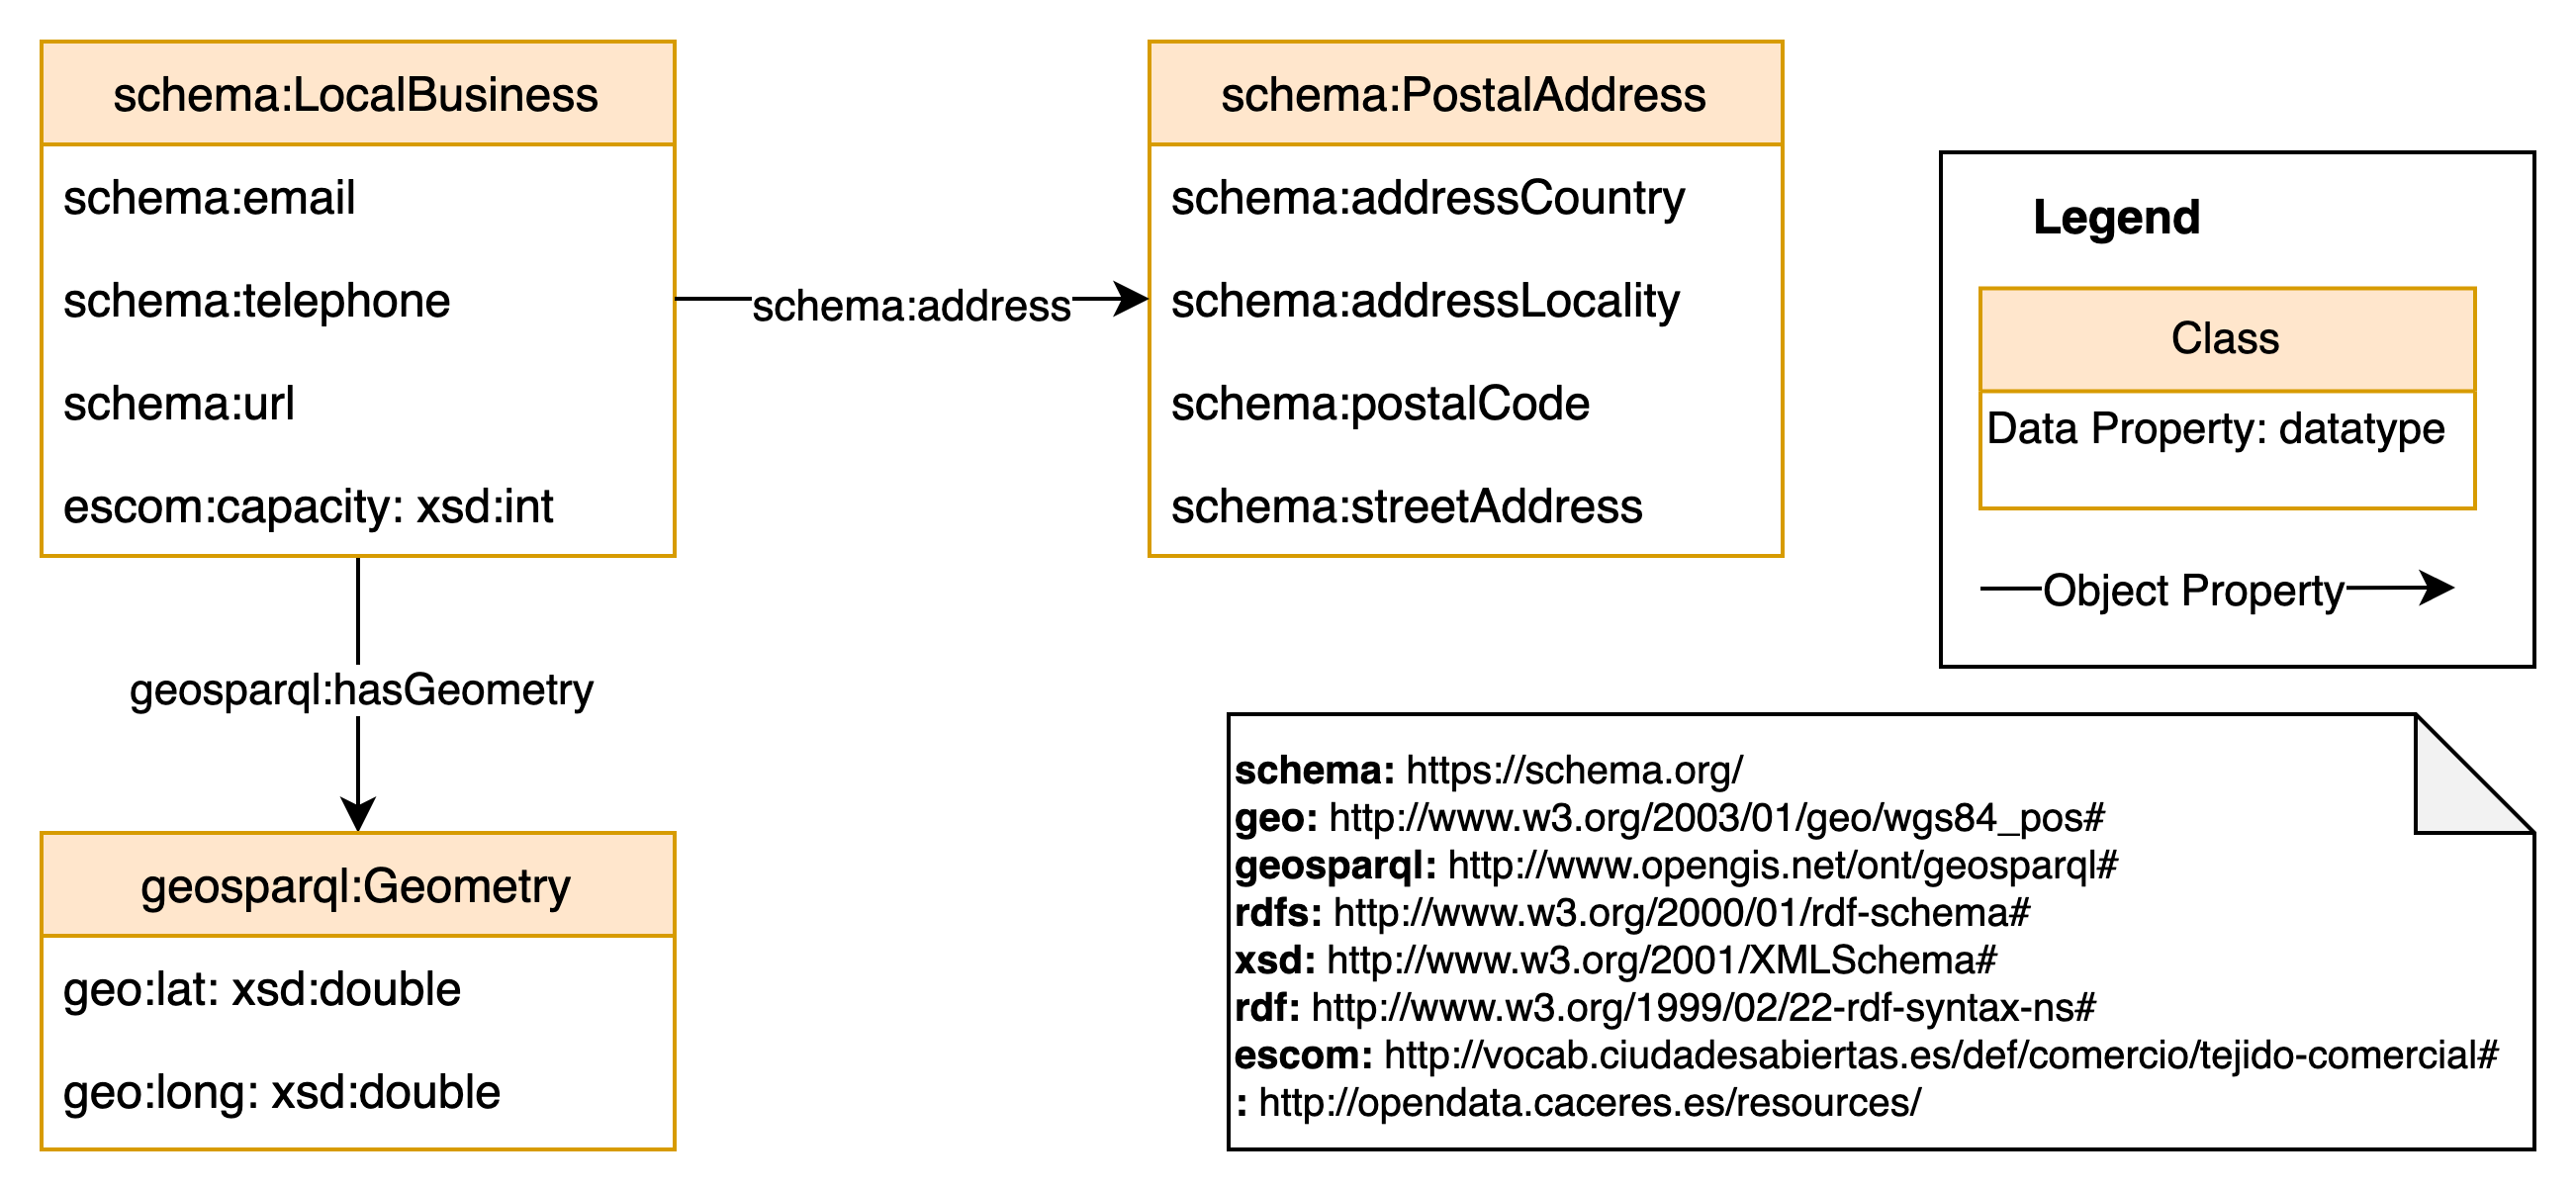
\includegraphics[width=\linewidth]{figures/chp5-1_us_onto.png}
\caption[Ontology diagram for the user study exercise of Mapeathor]{Ontology diagram representing a subset of the Vocabulary for data representation of the local business census and activities licenses.}
\label{fig:chp5-1_us_onto}
\end{figure*}

\noindent\textit{\textbf{Resources}}
The same data and ontology was used for both evaluations. We use a subset of the \textit{Vocabulary for data representation of the local business census and activities licenses}\footnote{\url{http://vocab.ciudadesabiertas.es/def/comercio/tejido-comercial/index-en.html}} that represents local businesses, their postal address and geolocalization (\cref{fig:chp5-1_us_onto}). 
We chose this dataset, that belongs to the common-knowledge domain, to avoid heterogeneous prior domain knowledge influence on the results of the study.

We provided participants with the subset ontology description and associated data, that is comprised of three CSV files: \texttt{bar.csv}, \texttt{restaurant.csv} and \texttt{address.csv}. Information about bars, restaurants and their geolocalization is represented in the files \texttt{bar.csv}, \texttt{restaurant.csv} respectively. 
These files contain the same columns, but different data. The file \texttt{address.csv} represent the postal address of the businesses present in the other two files. 
The original data is available in GitHub\footnote{\url{https://github.com/CiudadesAbiertas/vocab-comercio-censo-locales/}}. 
To facilitate the exercise for participants, some data cleaning was performed over the original files, as well as translation to all columns form spanish to english. The used resources are published in Zenodo~\citep{iglesias-molina_2022_8154522}.



\noindent\textit{\textbf{Participants}} 
In the \textit{subjective evaluation}, 17 attendants submitted answers to the questionnaire provided during the session. Most of the participants were knowledgeable in linked data, while less than half had already used mappings before. 
In the \textit{objective evaluation}, 30 participants were sampled from the Ontology Engineering Group, ranging from MSc students to full professors. Their background ranged from having basic knowledge about linked data and mappings, to being knowledgeable practitioners, including participants that were experts in linked data but had no knowledge about mappings. Prior to the assignation of participants to each group, participants were asked to provide information about whether they had prior knowledge of any of the tools, so that no participant would use a tool which they were already familiar with. Taking into account this restriction, they were randomly divided into three groups, one per tool. Each group was balanced w.r.t. the heterogeneity in background (\cref{fig:chp5-1_expertise}). 


\begin{figure*}[!t]
\centering
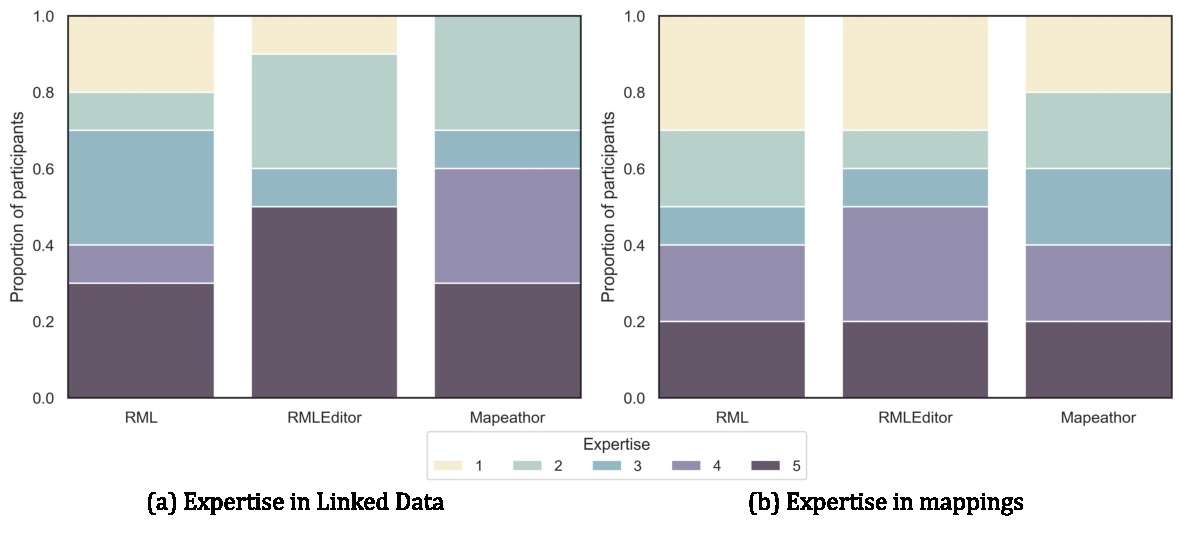
\includegraphics[width=1\linewidth]{figures/chp5-1_expertise.pdf}
\caption[Expertise of participants of the user study.]{Distribution of expertise of participants according to the 5-point Likert scale in (a) Linked Data and (b) mappings.}
\label{fig:chp5-1_expertise}
\end{figure*}

\noindent\textit{\textbf{Metrics}} 
The \textit{subjective evaluation} measured the responses to the SUS questionnaire on a 5-point Likert scale. 
For the \textit{objective evaluation},
%the accuracy of the mapping submitted was calculated. All participants had 30 minutes to perform the task and upload the resulting mapping, thus two kinds of accuracies are calculated. \ana{igual esta frase cuadrarla después }
we calculate two kinds of accuracies: (i)~\textit{Total Accuracy} (TA) for the number of correct rules written w.r.t. the reference correct mapping, and (ii)~\textit{Local Accuracy} (LA) for the number of correct rules w.r.t. all the written rules. We calculate both accuracies because of the fixed time for completing the exercise. TA can be interpreted as a measure of completeness, while LA focusses on assessing the correctness of the written rules independently on the total completeness.
We divide the mapping in four components: \textit{Subject}, \textit{Source}, \textit{Predicate-Object (PO)} and \textit{Join}, and calculate the accuracy for each component and the totality of the mapping. Then a T-Test is performed to look for significant differences of accuracy among the tools. This test is sed under the assumptions of (i) normality, (ii) sameness of variance, (iii) data independence, and (iv) variable continuity.


\noindent\textit{\textbf{Threats to validity}}~\citep{creswell2017research} We identify the following internal and external threats to the validity of our experiment.

\textbf{Internal validity threats} concern the experimental setup or experience of participants which threaten the ability to draw correct conclusions about the population in the experiment. We identify three internal threats: \textit{tool familiarity bias}, \textit{selection bias} and \textit{instruction bias}.
\begin{itemize}
    \item \textbf{Tool familiarity bias.} Practitioners tend to be more expert in some specific technologies and languages that they use more frequently. Thus, in the sample there it is possible to have participants that have used any of the tested approaches, which in turn can influence the results. For creating the groups, participants' experience was inquired to avoid assigning them a tool that they had previously used.
    \item \textbf{Selection bias.} The sample includes participants with different range of skills and previous knowledge about linked data and mappings. We mitigate this threat by defining groups that were  homogeneous w.r.t. range of expertise in mappings and linked data, considering also the mitigation measures for the \textit{tool familiarity} threat. That is to say, all groups included from beginner users to knowledgeable practitioners. 
    \item \textbf{Instruction bias.} One of the evaluated approaches is designed by the conductors of the user study. This situation could incur in bias on information delivery. To mitigate this threat, we provided participants with the same instruction guidelines for each tool. Three sessions were conducted subsequently to provide the same explanations and attention to each tool. During each sessions, all questions were answered with equal level of detail and guidance for all tools and participants.
\end{itemize}

\textbf{External validity threats} occur when wrong inferences from sample data are made beyond the studied sample or experimental setup. We identify two external threats: \textit{background of participants sample} and \textit{environment}.
\begin{itemize}
    \item \textbf{Background of participants sample.} This threat concerns the generalization to individuals outside the study. The sample of participants include a wide range in the variety of backgrounds, from not very familiar with linked data and mappings, to expert practitioners. We deliberately choose to have this variety for each group so that the results can be generalized to a broader sample, while mitigating the risks of internal threats described above that this choice poses. 
    \item \textbf{Environment.} This threat concerns the generalization to individuals outside the experiment’s setting. Participants were free to use a computer, browser and tools of their choice. Thus, they could perform the tasks required for the study in a well-known environment. No specific experimental setup prevents generalizations to individuals outside our study.
\end{itemize}




\subsubsection{Results}
\label{sec:chp5_mapeathor_results}

\noindent\textit{\textbf{Subjective evaluation results}}


\begin{table}[!t]
\caption{Results of the user study, showing the mean of the local accuracy (LA), total accuracy (TA) and p-value of the submitted responses per mapping feature and tool. }
\label{tab:chp5-1_summary_results}
\centering
\resizebox{\columnwidth}{!}
{\begin{tabular}{ccc|cc|cc|cc|cc}
    \cmidrule{2-11}
    & \multicolumn{2}{c|}{\textbf{Subject}} & \multicolumn{2}{c|}{\textbf{Source}} & \multicolumn{2}{c|}{\textbf{PO}} & \multicolumn{2}{c|}{\textbf{Join}} & \multicolumn{2}{c}{\textbf{Total}} \\ \cmidrule{2-11}
    & LA & TA & LA & TA & LA & TA & LA & TA & LA & TA \\ \midrule
    \textbf{\makecell{RML}} & 0.617 & 0.457 & 0.927 & 0.570 & \underline{0.684} & 0.458 & \underline{0.133} & \underline{0.150} & \underline{0.693} & 0.410  \\ \midrule
    \textbf{\makecell{RMLEditor}} & \underline{0.465} & \underline{0.360} & \underline{0.860} & \underline{0.560} & 0.705 & \underline{0.363} & 0.233 & 0.217 & 0.705 & \underline{0.340}  \\ \midrule
    \textbf{Mapeathor} & \textbf{0.858} & \textbf{0.620} & \textbf{0.960} & \textbf{0.620} & \textbf{0.795} & \textbf{0.581} & \textbf{0.250} & \textbf{0.225} & \textbf{0.831} & \textbf{0.547}  \\\midrule \midrule
    \textbf{p-value} & 0.090 & 0.295 & 0.596 & 0.890 & 0.777 & 0.337 & 0.746 & 0.881 & 0.476 &  0.264 \\ \bottomrule
\end{tabular}}
\end{table}

\noindent\textit{\textbf{Objective evaluation results}}

%\ana{e ir intercalando opiniones sobre cada approach para apoyar los resultados, ambas buenas y malas}
%\ana{de rmleditor fallos a nivel técnicos, opiniones divididas entre intuitivo/antiintuitivo, hay constructos que hay que explicar, pero una vez superada esa barrera medianamente bien. Remarcan que faltan funcionalidades como copy/paste de secciones enteras, y buscar mejor lo creado en el espacio de trabajo (a muchos se les perdían las cosas y había que volver a empezar)}
%\ana{de rml igual hay mejores resultados porque una vez se entienden las partes del mapping y partiendo de un ejemplo, qué hay que copiar y cambiar, eso agiliza el proceso. Más indicado para desarrolladores (más acostumbrados a escribir código), se señala que no es excesivamente complejo pero con alguna herramienta se haría mejor.}
%\ana{curva de aprendizaje de la herramienta, como todos, pero en general gusta que se pueda usar algo tan común como excel, que facilita mucho la escritura de reglas. El punto negativo viene por el tema de los IDs, que al no aparecer automáticos en las subsecuentes pestañas induce a errores.}

%% In general
\cref{tab:chp5-1_summary_results} shows the results obtained from the user study. In general, it can be observed that Mapeathor obtains the highest accuracy rate in all cases. Surprisingly, RMLEditor struggles with the base approach, RML, obtaining in general slightly worse results. Between these two approaches, participants using RML were able to complete more total mapping rules, while for RMLEditor the written rules were more accurate. 

%% no significance, but tendencies in differences in parts
However, none of the differences in the results for any type of mapping rule is significant (p-values $>$ 0.05), but we can observe some tendencies. The results for which the p-value is closer to being significant is for the total accuracy of the complete mapping, and for the subjects (specially its local accuracy). In this cases, it can be stated with more confidence that Mapeathor can help the writin process. 
%\textit{sin embargo, ninguno de los resultados es significativo (p-value $<$ 0.05), pero sí se pueden observar tendencias. Los resultados donde más se acerca el p-value a ser significativo es para el total accuracy del mapping completo, y para la escritura de los sujetos, especialmente en el local accuracy. En estos casos se puede afirmar con más seguridad que Mapeathor va bien encaminado a mejorar la escritura de las mapping rules.}  \ana{de donde rmleditor supera a rml tb?}

%% analysis of parts of mappings
Looking at the details of each mapping parts, in general the writing of \textit{Sources}, \textit{Subjects} and \textit{Predicate-Object} pairs (\textit{PO}) is carried out mostly successfully. It is especially remarkable for \textit{Sources}, that achieves a local accuracy near to 1. However, the results reported for its total accuracy are not that high, which can be due to the time limit and the increasing complexity of the exercise. The accuracy of the creation of \textit{Subjects} with the RMLEditor is rather low w.r.t the other approaches. \ana{detalle de los fallos comunes para este caso, mirar mappings directamente}. The mapping element where all approaches fail to assist users is unmistakably the \textit{Joins}. Most participants did not even try to write them, and those who did mostly failed. 

%\textit{mirando más en detalle a cada una de las partes del mapping, se puede ver que en general la escritura de sujetos, sources y poms es muy exitosa, sobre todo de los sources, donde el local accuracy de todos los approaches es cercanoa 1. regarding el total accuracy, los resultados no son tan buenos, en parte puede ser por el tiempo dado, y en parte por la complejidad incremental del mapping. que había dos sujetos creados a partir del mismo archivo, y dos archivos que servian para crear el mismo sujeto. Donde todas las herramientas fallan estrepitosamente es en la creación de joins, llevandose la palma RML. Aquí si se puede ver que los user-friendly approaches si apoyan a la escritura, pero sin mucho éxito tampoco.}


%% en general



\begin{figure}[t!]
    \centering
    \begin{subfigure}[b]{\linewidth}
    	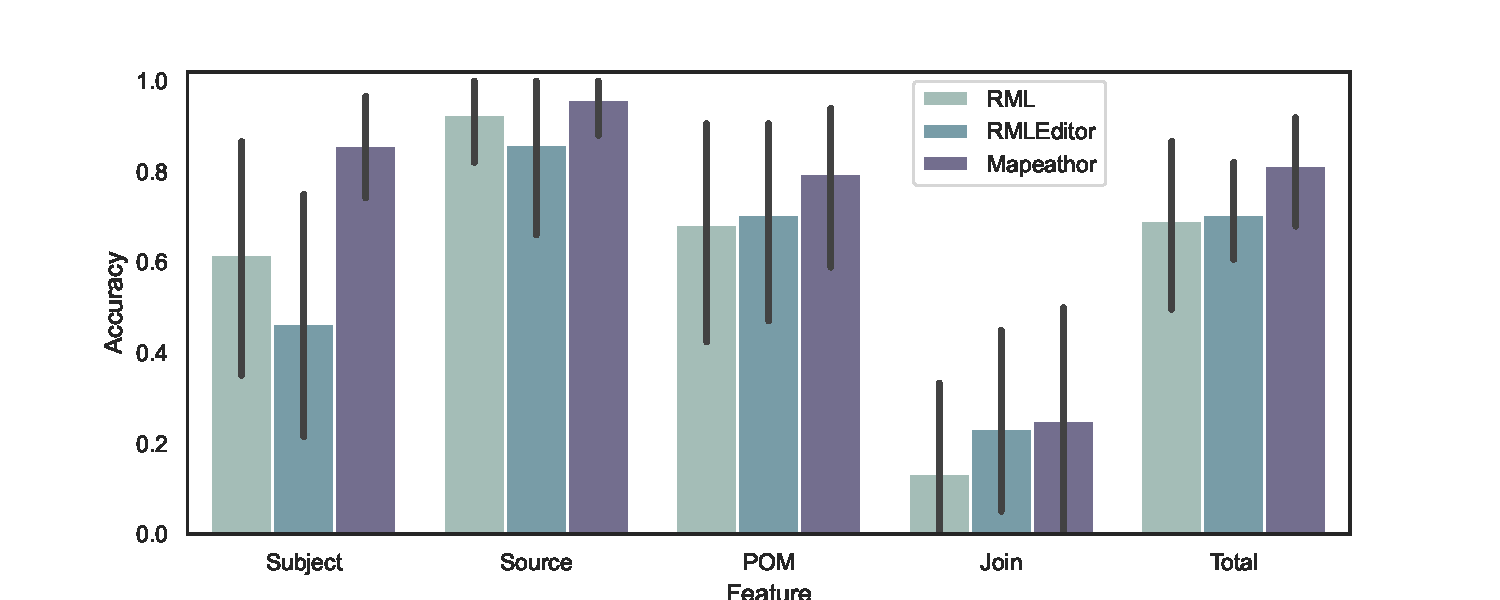
\includegraphics[width=\linewidth]{figures/mapeathor_rel-acc.pdf}
    	\caption{Local accuracy.}
    	\label{fig:chp5_mapeathor_relacc}
    \end{subfigure}
   %\hspace{0.05\textwidth}
    \begin{subfigure}[b]{\linewidth}
    	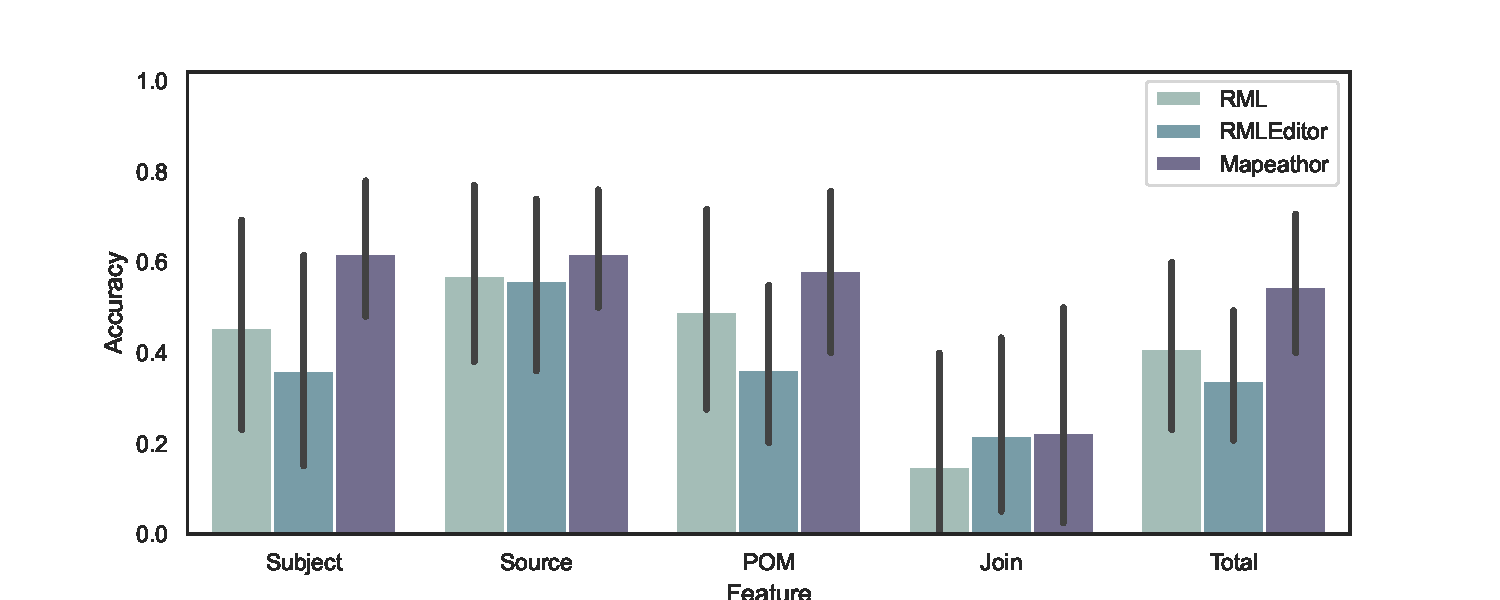
\includegraphics[width=\linewidth]{figures/mapeathor_total-acc.pdf}
    	\caption{Total accuracy.}
    	\label{fig:chp5_mapeathor_totacc}
    \end{subfigure}
    \caption{Accuracy results.\ana{estando la tabla esto queda redundante?}}
    \label{fig:reification-app}
\end{figure}


%\subsection{Use cases}
%Ciudades abiertas, EBOCA, photocatalisis ontology
%\ana{bueno ya veremos}



\subsection{Discussion}
\label{sec:chp5_mapeathor_discussion}
\ana{discusión de resultados, y use cases también se pueden comentar. O al igual si no es mucho se puede decir directamente en las conclusiones del capítulo}

In general, the results obtained in the user study show that there is still plenty of room for improvement for facilitating the adoption and use of mappings by a broader community of users. In each group, there were participants able to completely finish the exercise on time. In addition, plenty other participants claimed (in the feedback space left in the questionnaire) that, without the time limit, it would have been possible for them to complete the mappings. However, the reported local accuracy indicates that, even complete, the mapping would not have been entirely valid. This success rate holds true both for new users as well as for people with expertise on other mapping technologies. 

It is specially remarkable the results obtained for the RMLEditor, that overall does not improve the results of RML. These results seem to be a product of the technological support rather than the visual notation. Multiple participants using the RMLEditor stress the lack of certain functionalities, like the impossibility of copying and pasting sections of the created mapping, and the difficulty of finding created mapping constructs in the working space. The contrary was reported for RML, where participants, once they understood the parts that they had to copy and modify, it got easier for them to complete the mapping rules. Regarding Mapeathor, multiple participants highlighted that using spreadsheets was convenient for them to carry out the exercise. The flaw most pointed out, however, was the need to separate the rules in different sheets. Specially for the creation and tracking of the ruleset's \texttt{ID}, participants missed an automated way of filling this ID with the ones created in other sheets. As the process is currently manual, it can induce to errors.

Hence, we can observe that developing tools that aid the mapping writing is generally desired, and can improve the process both by (i) speeding up the writing and (ii) ensuring that the rules written produce correct mapping documents. The higher accuracy reported by the participants using Mapeathor motivates that the spreadsheet-based approach is useful for this aim. Yet, there is still room for improvement regarding the cohesion of the sheets and the shared \texttt{IDs} across them, the potential for hosting more expresiveness from the ever-evolving mapping languages (\ana{refs ICWE and RML} and leveraging more spreadsheet funcionalities to improve the user experience. 

%\textit{en general los resultados (accuracy conseguido) dejan bastante que desear. Hay que tener en cuenta que los participantes tenían un tiempo limitado para terminar el ejercicio, pero aún así el mejor resultado de total accuracy (en total y en las partes) supera por poco la mitad del completeness. Para cada grupo hubo gente que consiguió terminar el ejercicio o se quedó muy cerca (al menos una persona por grupo). Mientras, fueron mayoría quienes completaron pocas reglas, de ahí que el local accuracy sea mejor. Sin embargo, este accuracy también nos dice que la mayoría de participantes tuvo dificultades para hacer el mapping, cosa que ocurrió para ambos gente que ya habían hecho mappings y nuevos usuarios. Estos resultados resaltan que queda mucho camino por recorrer para mejorar el proceso de creación y escritura de mappings. }

\ana{newpage hasta que la seccióne esté entera, borrar después}
\newpage

\section{User-friendly Creation of Mapping Rules for RDF-star with YARRRML}
\label{sec:chp5_yarrrml_star}

Along with mapping editors described before, human-friendly serializations emerged 
to ease the definition of mapping rules. Focusing on R2RML and RML, we highlight the following serializations that have been more widely adopted recently.
YARRRML~\parencite{Heyvaert2018yarrrml} leverages YAML
to offer a user-friendly representation to define mapping rules, while
ShExML~\parencite{Garcia-Gonzalez2020shexml} extends the syntax of the ShEx constraint language~\parencite{prud2014shex}.
XRM~\parencite{xrm}
provides an abstract syntax that simulates programming languages and 
SMS2~\parencite{sms2}, proposed by Stardog\footnote{\label{foot:stardog}\url{https://www.stardog.com/}}, is loosely based on the SPARQL query language and extends the features of R2RML to create virtual KGs.
Each serialization is accompanied by a system that translates their rules into mapping languages, such as RML or R2RML (henceforth abbreviated as [R2]RML). 
%These serializations and translators were not compared with each other in terms of serializations' features and system's characteristics, even though it would help to decide which serialization fits each use case.

This section describes YARRRML-star, the extension of YARRRML to support RML-star~\parencite{delva2021rml-star} to construct RDF-star graphs.
We also improve the serialization to adhere with the latest RML updates
(e.g., datatypes, joins, etc.), and develop a translator system --Yatter-- that implements the new features, and validate our proposal with test cases and compared it to other user-friendly serializations.

\subsection{User-friendly Syntax for Mapping Rules}
\label{sec:chp5_yarrrml-desc}
We extend the YARRRML serialization to support the RDF-star construction, two updates (dynamic datatypes and language tags), and a shortcut for join conditions. These are recent features in RML that so far were not considered in YARRRML.
To illustrate the extensions,
we use a CSV file as input (\cref{lst:chp5_csv}) with information about pole vaulters: an identifier, name, language of the country, height of the jump, date when the jump takes place, and type of date format specified.

\noindent\begin{minipage}{\linewidth}
\centering
\begin{captionedlisting}
{lst:chp5_csv}{Contents of the \texttt{jump-source} logical source.}
\centering
\begin{tabular}{c}
{\begin{lstlisting}[basicstyle=\ttfamily\small,columns=flexible]
ID , PERSON         , COUNTRY , MARK , DATE                       , DATE-TYPE
1  , Lisa Ryzih     , de       , 4.40 , 2022-03-21                , date
2  , Xu Huiqin      , zh       , 4.55 , 2022-03-19T17:23:37       , dateTime
\end{lstlisting}}
\end{tabular}
\end{captionedlisting}
\end{minipage}

\subsubsection{YARRRML-star} %Ana

 %\ana{ojo con repetir de qué va RDF-star, que en relwork y RML-star ya se dirá también)

RDF-star introduces the notion of RDF-star triples, i.e., triples that are subjects or objects of another triple. These triples are enclosed using ``\texttt{<<}'' and ``\texttt{>>}'', and can be (1) quoted, if they only appear in a graph embedded by another triple (List~\ref{lst:chp5_res-rdf-star} lines 2,4); or (2) asserted, if the quoted triple is also generated outside the triple where it is quoted (lines 1-4).
We extend YARRRML to specify how we can construct RDF-star graphs, aligned with the RML-star specification~\parencite{iglesias2022rmlstar}.

\begin{minipage}{\linewidth}
\centering
\begin{captionedlisting}{lst:chp5_res-rdf-star}{RDF-star triples.}
\centering
\begin{tabular}{c}
{\begin{lstlisting}[numbers=left,basicstyle=\ttfamily\small,columns=flexible]
:1 :jumps 4.40 .
<< :1 :jumps 4.80 >> :date "2022-03-21" .
:2 :jumps 4.55 .
<< :2 :jumps 4.85 >> :date "2022-03-19T17:23:37" .
\end{lstlisting}}
\end{tabular}
\end{captionedlisting}
\end{minipage}

RDF-star triples can be created in YARRRML-star (\cref{lst:chp5_mapping-star}) by referencing existing Triples Maps with the tags (1) \texttt{quoted} for quoted asserted triples (line 10) and (2) \texttt{quotedNonAss\-erted} for quoted non-asserted triples.  
% (see further examples in the specification\footnote{\url{https://dachafra.github.io/yarrrml-spec/#rdf-star}}. 
%Listing \ref{lst:chp5_mapping-star} shows an example of a YARRRML mapping that creates a quoted asserted triple from data in Listing \ref{lst:chp5_csv}. 
The triple that the rule set \texttt{jumpTM} creates is used as subject in the rule set \texttt{dateTM}, creating RDF-star triples (\cref{lst:chp5_res-rdf-star}). The equivalent mapping rules in RML are shown in \cref{lst:chp5_mapping-rml-star}.  

\begin{minipage}{\linewidth}
\centering
\begin{captionedlisting}{lst:chp5_mapping-star}{YARRRML-star mapping rules. }
\centering
\begin{multicols}{2}
{\begin{lstlisting}[numbers=left,basicstyle=\ttfamily\small,columns=flexible,language=yarrrmlstar]
mappings:
 jumpTM:
  sources: jump-source
  subjects: :$\dollar$(ID)
  predicateobjects:
   - [:jumps, $\dollar$(MARK)]
 dateTM:
  sources: jump-source
  subjects:
   quoted: jumpTM
  predicateobjects:
   - [:date, $\dollar$(DATE)]
\end{lstlisting}}

\end{multicols}
\end{captionedlisting}
\end{minipage}

\begin{minipage}{\linewidth}
\centering
\begin{captionedlisting}{lst:chp5_mapping-rml-star}{RML-star mapping rules translated from \cref{lst:chp5_mapping-star}. }
\centering
\begin{multicols}{2}
{\begin{lstlisting}[numbers=left,basicstyle=\ttfamily\small,columns=flexible,language=rmlstar]
<#jumpTM> 
  a rml:AssertedTriplesMap ;
  rml:logicalSource :jump-source;
  rml:subjectMap [ 
    rr:template ":{ID}" ] ;
  rr:predicateObjectMap [ 
    rr:predicate :jumps ;
    rml:objectMap [
      rml:reference "MARK" ] ] .
<#dateTM> 
  a rr:TriplesMap ;
  rml:logicalSource :jump-source ;
  rml:subjectMap [ 
    rml:quotedTriplesMap <#jumpTM> ];
  rr:predicateObjectMap [ 
    rr:predicate :date ;
    rml:objectMap [
      rml:reference "DATE" ] ] .
\end{lstlisting}}

\end{multicols}
\end{captionedlisting}
\end{minipage}





\subsubsection{Additional Updates} %Ana
%The resulting triples (Listing \ref{lst:chp5_res-lang}) present a different language tag and datatype according to the input data source (Listing \ref{lst:chp5_csv}). The equivalent mapping in RML is presented in Listing \ref{lst:chp5_mapping-lang-rml}.
%We add a new feature to comment terms in the mapping. These comments can be added to sources, subjects and predicate-object maps. 
%Comments start with ``\texttt{\#}" and contain a \texttt{TITLE} and \texttt{COMMENT} separated by ``\texttt{|}" (Listing \ref{lst:chp5_mapping-comment}). 
%They are translated into RML to two properties: \texttt{rdfs:label} for \texttt{TITLE} and \texttt{rdfs:comment}  for \texttt{COMMENT} (Listing \ref{lst:chp5_rml-comment}).
We enable YARRRML-star with other new features that have been incorporated into RML in recent years. 
%Listing \ref{lst:chp5_yarrrml-updates} shows the updates and the translation to RML is shown in Listing \ref{lst:chp5_rml-updates}. 
%The first additional update we highlight is the possibility of 
We extend YARRRML to assign datatypes and language tags dynamically to objects. 
They are generated with the data values, in the following examples the datatype is generated dynamically with the data field \texttt{DATA-TYPE} (\cref{lst:chp5_dyn_datatype}), and the language tag with \texttt{COUNTRY} (\cref{lst:chp5_dyn_lang}). They translate into RML as Listings \ref{lst:chp5_dyn_datatype_rml} and \ref{lst:chp5_dyn_lang_rml} show.




\begin{minipage}{0.45\linewidth}
\begin{captionedlisting}{lst:chp5_dyn_datatype}{Dynamic datatype in YARRRML-star.}
\centering
\begin{tabular}{c}
\hspace{-3em}
{
\begin{lstlisting}[basicstyle=\ttfamily\small,columns=flexible,language=yarrrmlstar]
- [:date, $\dollar$(DATE), xsd:$\dollar$(DATE-TYPE)]
\end{lstlisting}
}
\end{tabular}
\end{captionedlisting}
\end{minipage}
\,\,\,\,\hfill
\begin{minipage}{0.45\linewidth}
\begin{captionedlisting}{lst:chp5_dyn_lang}{Dynamic language tag in YARRRML-star.}
\centering
\begin{tabular}{c}
\hspace{-2.5em}
{
\begin{lstlisting}[basicstyle=\ttfamily\small,columns=flexible,language=yarrrmlstar]
- [:name, $\dollar$(PERSON), $\dollar$(COUNTRY)~lang]
\end{lstlisting}
}
\end{tabular}
\end{captionedlisting}
\end{minipage}








\begin{minipage}{0.45\linewidth}
\begin{captionedlisting}{lst:chp5_dyn_datatype_rml}{Dynamic datatype in RML translated from \cref{lst:chp5_dyn_datatype}.}
\centering
\begin{tabular}{c}
\hspace{-1em}
{
\begin{lstlisting}[numbers=left,basicstyle=\ttfamily\small,columns=flexible,language=rmlstar]
rr:predicateObjectMap [ 
 rr:predicate :jumpsOnDate ;
 rml:objectMap [
  rml:reference "DATE";
  rml:datatypeMap [
   rr:template "xsd:{DATE-TYPE}"]]];
\end{lstlisting}
}
\end{tabular}
\end{captionedlisting}
\end{minipage}
\,\,\,\,\hfill
\begin{minipage}{0.45\linewidth}
\begin{captionedlisting}{lst:chp5_dyn_lang_rml}{Dynamic language tag in RML translated from \cref{lst:chp5_dyn_lang}.}
\centering
\begin{tabular}{c}
\hspace{0.5em}
{
\begin{lstlisting}[numbers=left,basicstyle=\ttfamily\small,columns=flexible,language=rmlstar]
rr:predicateObjectMap [ 
 rr:predicate :name ;
 rml:objectMap [
  rml:reference "PERSON";
  rml:languageMap [
   rml:reference "COUNTRY"]]];
\end{lstlisting}
}
\end{tabular}
\end{captionedlisting}
\end{minipage}


We also incorporate a shortcut for specifying join conditions (\cref{lst:chp5_join}). This shortcut follows the functions' syntax\footnote{\url{https://rml.io/yarrrml/spec/\#functions}}. %, and translates to normal join conditions in RML (\cref{lst:chp5_rml-mapping} lines 16-22)
It is specified as the function \texttt{join} that takes as parameters the mapping identifier (with the \texttt{mapping=} parameter key) and the similarity function to perform the join. 
This function can, in turn, take data values as parameters. 
Quoted and non-asserted triples can also be generated within join conditions by using the parameter keys \texttt{quoted=} and \texttt{quotedNonAsserted=} respectively.
In the example, the join condition is performed using the \texttt{equal} function to create as objects the subjects of the mapping set \texttt{jumpTM} if the values of the fields \texttt{ID} from source and \texttt{ID} from target mapping set are the same.

%All the described updates have been proposed for the YARRRML specification and are currently under review by the KG Construction Community Group\footnote{\url{https://github.com/kg-construct/yarrrml-spec/pull/4}}.

\begin{minipage}{\linewidth}
\centering
\begin{captionedlisting}{lst:chp5_join}{Abbreviated syntax for join conditions in YARRRML-star.}
\centering
%\begin{multicols}{2}
{\begin{lstlisting}[numbers=left,basicstyle=\ttfamily\small,columns=flexible,language=yarrrmlstar]
- predicates: :jumps
  objects:
   - function: join(mapping=jumpTM, equal(str1=$\dollar$(ID), str2=$\dollar$(ID)))
\end{lstlisting}}
%\end{multicols}
\end{captionedlisting}
\end{minipage}





\subsection{Implementation: Yatter}

%In this section, we describe 
Yatter\footnote{\label{foot:yatter}\url{https://github.com/oeg-upm/yatter/}} is a bi-directional YARRRML translator that supports the features described in previous sections. 
Yatter receives as input a mapping document in the YARRRML serialization and the desirable output format (R2RML or RML), or the other way around.




\cref{alg:yatter} presents the procedure implemented by the system to translate an input YARRRML mapping document into [R2]RML. 
First, %prefixes are added (
the namespaces defined in YARRRML are added together with a set of predefined ones (e.g., \texttt{foaf\footnote{\url{http://xmlns.com/foaf/0.1/}}, rml\footnote{\url{http://semweb.mmlab.be/ns/rml\#}}, rdf\footnote{\url{http://www.w3.org/1999/02/22-rdf-syntax-ns\#}}}) that are used in by [R2]RML. 

Second, functions, targets, and databases are identified in the entire YARRRML document and translated into RML. Each of them generates a global identifier mapped into a hash table that can be used by any \texttt{rr:TermMap}. For external source declaration, their identifiers are also mapped into a hash table for the next steps.
Regarding the RDF-star support, the mapping rules are parsed to identify if it contains \texttt{quoted} or \texttt{quotedNonAsserted} keys.
This determines if the translation requires producing RML-star mapping rules.
If true, a hash table is also created for the mapping instances of \texttt{rml:NonAssertedTriplesMap}.


In YARRRML, lists of sources and subjects maps can be defined within the same triples map, but [R2]RML triples maps may contain only one source and one subject. 
Hence, for each mapping document, a list of sources and subjects is first collected and then translated depending on the desirable output format ([R2]RML[-star]). 
Nevertheless, multiple predicate maps and object maps are allowed within the same triples map, and they are directly translated to RML.
Finally, the cartesian product of sources and subject maps together with the predicate object maps is combined to generate the desirable triples map.
Before returning the mapping rules, Yatter validates that the generated output is a valid RDF graph.


\begin{minipage}{0.95\linewidth}
\begin{algorithm}[H]
\SetAlgoLined
\KwResult{[R2]RML mapping document}
 $input\_m \longleftarrow yarrrml\_rules$\;
 $format \longleftarrow output\_format$\;
 $output\_m \longleftarrow \emptyset$\;
 
 $output\_m.add(translate\_prefixes(input\_m))$\;
 \If{$format == RML$}{
    $output\_m.add(translate\_functions(input\_m))$\;
    $output\_m.add(translate\_targets(input\_m))$\;
    $is\_star, non\_asserted\_maps \leftarrow analyze\_rml\_star(input\_m)$\;
 }   
 $output\_m.add(translate\_databases\_access(input\_m))$\;
 $ext\_sources \leftarrow get\_external\_sources(input\_m)$;
 
 \For{$tm \in M.get\_triples\_map()$}{
    $source\_list \leftarrow translate\_source(format, get\_source\_list(ext\_sources, tm))$\;
    $subject\_list \leftarrow translate\_subject(is\_star, format, get\_subject\_list(tm))$\;
    $predicates\_objects \leftarrow translate\_predicates\_objects(is\_star, format, tm)$\;
    \For{$s \in source\_list$}{
        \For{$subj \in subject\_list$}{
            $m \leftarrow combine(s, subj, predicates\_objects, non\_asserted\_maps))$\;
            $output\_m.add(m)$\;
        }
    }
 }
 \Return{$validate(output\_m)$}\;
\caption{YARRRML-star translation algorithm}
\label{algorithm-yatter}
\end{algorithm}
\end{minipage}

Although YARRRML leaves the RDF-based syntax of the mapping rules to be processed only by the knowledge graph construction systems, we also provide a human-readable output in the same way as Mapeathor does (see \cref{sec:chp5_mapeathor_tool}). 
Moreover, we ensure that functions, targets, and databases appear first, while for each \texttt{rr:TriplesMap}, the sequence is: source, subject map, and the set of predicate object maps.

The source code of Yatter is openly available under an Apache 2.0 license\cref{foot:yatter}.
Following open science best practices, each release automatically generates a dedicated DOI to ensure reproducibility in any experimental evaluation\footnote{\url{https://doi.org/10.5281/zenodo.7024500}}. 
The development is under continuous integration using GitHub Actions and the YARRRML test-cases (Section \ref{sec:chp5_yarrrml-validation}) have more than 80\% code coverage. 
Yatter is available through PyPi as a module\footnote{\url{https://pypi.org/project/yatter/}}~\parencite{david_chaves_2024_yatter} to be easily integrated in any Python development. % (e.g., providing RML to a KG construction system implemented in this language).
%such as SDM-RDFizer~\parencite{iglesias2020sdm} or Morph-KGC~\parencite{arenas2022morph}.



\subsection{Validation}
\label{sec:chp5_yarrrml-validation}
We validate the extensions to YARRRML and the developed implementation by 
proposing and testing a set of test cases, and comparing to other proposed user-friendly serializations and corresponding systems.

\subsubsection{YARRRML Test Cases} %David
Test cases are a common method to evaluate the conformance of a system~\parencite{arenas2023morphstar,heyvaert2019conformance}. 
%with respect to a language/syntax specification 
%(see for example). 
To the best of our knowledge, previous R2RML~\parencite{boris2012r2rml} and RML~\parencite{heyvaert2019conformance} test cases were not translated to any human-friendly serialization (e.g., YARRRML).
Relying on [R2]RML test cases, we propose a set of representative test cases (including also the new features presented in this work) to assess the conformance of any YARRRML translator system.
%In this way, practitioners can easier understand the coverage of these systems with respect to the proposed language/syntax and select the one that fits better to their own use cases.
The proposed test cases serve two objectives, (i) to cover the complete vocabulary of the serialization, and (ii) to have the flexibility to declare the rules (e.g., shortcuts or location of the keys). 
%To avoid starting from scratch, we rely on the test cases proposed by R2RML~\parencite{R2RML_test_cases} first, that were also extended for RML~\parencite{heyvaert2019conformance}. 

We follow a systematic methodology for creating the YARRRML test cases. 
We analyzed the [R2]RML test cases and observed that several assess correct data generation.
Since YARRRML serves as user-friendly serialization for another mapping language, the focus of its test cases is not on assessing data correctness, but on covering the language expressiveness.
Hence, we select 15 R2RML test cases that cover the R2RML features and manually translate them into YARRRML. 
%the flexiblity in rules declaration in YARRRML (i.e., to test proper manage of shortcuts).
Since RML is a superset of R2RML, it introduces modifications with respect to R2RML to include the definition of heterogenous datasets (e.g., \texttt{rr:LogicalTable} is superseded by \texttt{rml:LogicalSource}). % with their associated properties (e.g., \texttt{rml:source}), and \texttt{rr:column} by \texttt{rml:reference}.
We propose 8 new test cases to cover these features. 

For features not covered by the RML test cases, we follow a similar procedure. 
We inspected the RML-star test cases~\parencite{david_chaves_2022_6518802}, and translated to YARRRML the ones that provide a complete coverage of this extension. 
From the 16 test cases proposed to assess the conformance of RML-star, we adapt 6. 
Finally, we propose 21 test cases to cover RML-Target, RML-FNML, RML dynamic language tags and datatypes. 
%analyze both of each specifications (RML and YARRRML) and 
%we proposed another 21 test cases to cover them.

In total, we defined 50 YARRRML test cases and their corresponding translation to RML or R2RML. 
They are openly available\footnote{\label{foot:yarrrml-resources}\url{https://github.com/oeg-upm/yarrrml-validation}} to be used by any YARRRML-compliant system.
Yatter passes all test cases successfully. %Following good software development practices, we integrate the test cases in the continuous integration pipeline of our system as unit tests.


\subsubsection{Serializations Comparison} %Ana

%YARRRML was developed to be a user-friendly syntax for the RML mapping language~\parencite{heyvaert2018yarrrml}. There have been proposed more syntaxes with the same purpose, such as Stardog's SMS2 for R2RML and Zazuko's XRM for [R2]RML and CSVW.




We compare a set of user-friendly serializations and languages, namely SMS2~\parencite{sms2}, XRM~\parencite{xrm}, ShExML~\parencite{Garcia-Gonzalez2020shexml} and YARRRML~\parencite{Heyvaert2018yarrrml} incorporating the updates described in \cref{sec:chp5_yarrrml-desc}, regarding their expressiveness. 
To that end, we study 15 features that tackle usual characteristics and functionalities in mapping languages.
We describe each and discuss how each serialization addresses it (\cref{tab:chp5_lang-comparison}). 

\textbf{LF1. Subject Term Type.} 
This feature indicates what kind of RDF[-star] term the language can generate as subject.
In RDF, subjects can be IRIs or blank nodes, while in RDF-star they can also be RDF-star triples.
All serializations enable the creation of subjects at least as IRIs, SMS2 and YARRRML additionally implement RDF-star triples and, along with ShExML, blank nodes.

\textbf{LF2. Subject Generation.} 
This feature indicates if subjects can be generated as constant or dynamic values; and how many subject declarations are allowed at a time. In dynamically generated values, the subject value changes with a field in the data source. In our example, the subject uses the field ``\texttt{ID}" to generate different subject for each row of input data. %(\cref{lst:chp5_yarrrml-mapping} line 6) . Esto viene de la sección de background, que por ahora no voy a incluir
All serializations can generate constant and dynamic subjects. For each set of rules, exactly one subject declaration is expected, i.e., one subject for predicate-object pairs. YARRRML can also accept no subject declaration, producing a blank node. % as default behavior.
%whose default behavior generates a blank node when a subject is not described.


\begin{table}[t!]
\caption[Features of user-friendly serializations]{Features of user-friendly serializations. BN stands for blank node, L for literal, ST for RDF-star triple, C for constant and D for dynamic. \underline{Underlined} features indicate the updates of YARRRML-star, while
``*'' indicates that a feature is possible with the implementation but not explicit in the serialization.}
\label{tab:chp5_lang-comparison}
%\def\arraystretch{1.25}
\centering
\resizebox{0.8\columnwidth}{!}{
\begin{tabular}{r|cccccc}
 & \textbf{ShExML} & & \textbf{SMS2} & & \textbf{XRM} & \textbf{YARRRML-star} \\ \midrule
\textbf{LF1}& BN, IRI & & BN, IRI, ST & & IRI& BN, IRI, \underline{ST}\\ \midrule
\textbf{LF2}& C, D (1..1) & & C, D, (1..1) & & C, D, (1..1) & C, D (0..1)\\ \midrule
\textbf{LF3}& IRI & & IRI & & IRI & IRI\\ \midrule
\textbf{LF4}& C (1..1) & & C, D (1..1) & & C (1..1) & C, D (1..N)\\ \midrule
\textbf{LF5} & BN, IRI, L & & BN, IRI, L, ST & & IRI, L & BN, IRI, L, \underline{ST} \\ \midrule
\textbf{LF6} & C, D (1..1) & & C, D (1..N) & & C, D (1..1) & C, D (1..N)\\ \midrule
\textbf{LF7} & C, D (0..1) & & C (0..1) & & C (0..1) & C, \underline{D} (0..1)\\ \midrule
\textbf{LF8}& C, D (0..1) & & C, D (0..1) & & C (0..1) & C, \underline{D} (0..1)\\ \midrule
\textbf{LF9}& C (0..1) & & C (0..1) & & C, D (0..N) & C, D (0..N)\\ \midrule
\textbf{LF10} & (1..N) & & (1..N) & & (1..N) & (1..N)\\ \midrule
\textbf{LF11} & Input & & Input & & Input & Input, output\\ \midrule
\textbf{LF12} & \checkmark & & \xmark* & & \xmark* & \checkmark\\ \midrule
\textbf{LF13}& \checkmark & & \xmark & & \xmark & \xmark \\ \midrule
\textbf{LF14} & \checkmark & & \checkmark & & \xmark & \checkmark\\ \midrule
\textbf{LF15}& \checkmark & & \xmark & & \xmark & \checkmark\\ \midrule
\end{tabular}
}
\end{table}


\textbf{LF3. Predicate Term Type.} 
This feature indicates if the serialization is able to generate an IRI for a predicate and all serializations do so.

\textbf{LF4. Predicate Generation.}
This feature indicates if predicates can be generated as constant or dynamic values; and how many predicate declarations are allowed at a time. In dynamically generated values, the subject value changes with a field in the data source. 
%can be generated as constant values or change dynamically with the data iteration; and how many predicates declarations are allowed at a time. 
SMS2 and YARRRML enable dynamic predicates, and YARRRML is also able to handle more than one predicate, which avoids repeating the same object for different predicates.

\textbf{LF5. Object Term Type.} 
This feature indicates what kind of RDF[-star] term the serialization is able to generate as object. The serializations can generate the same kinds of terms as in subjects (LF1), with the addition of literals. 

\textbf{LF6. Object Generation.}
This feature indicates if objects can be generated as constant or dynamic values; and how many predicate declarations are allowed at a time.
%can be generated as constant values or change dynamically with the data iteration; and how many objects declarations are allowed at a time. 
As for subjects, all serializations can generate constant and dynamic objects. In addition, SMS2 and YARRRML allow more than one at a time, which avoids repeating the same predicate for different objects.

\textbf{LF7. Datatype.}
This feature indicates if datatypes can be specified constant or dynamically.
All serializations enable the optional declaration of constant datatypes, but ShExML and YARRRML also enable dynamic datatypes.

\textbf{LF8. Language Tag.}
This feature indicates if language tags can be constant or dynamic. Just as for datatypes, all serializations enable the optional declaration of constant language tags, XRM is the only not allowing dynamic.

\textbf{LF9. Named Graph.} 
This feature indicates if named graphs can be assigned to the generated statements and how (constant or dynamically). 
All serializations enable their optional declaration as constant IRI. XRM and YARRRML also enable more than one graph assignation, and allow dynamic values. 

\textbf{LF10. Data references.} 
This features indicates how many data references a term can contain when generated dynamically (i.e., when its value changes with the input data). It applies to subjects, predicates, objects, datatypes, language tags and named graphs when the serialization allows dynamic generation. All serializations allow more than one data reference for dynamic generation.

\textbf{LF11. Data Description.}
This feature indicates if the input or output data (e.g., format, iteration, name, path, etc.) can be described. All serializations can describe input data source, and YARRRML also provides the output data source.

\textbf{LF12. Data Linking.}
This feature indicates if explicit data linking (e.g., join, fuzzy linking, etc) can be performed with mapping rules. ShExML and YARRRML provide specific features for this end; in XRM and SMS2, however, it is not explicit, but it is possible by using SQL queries. 

\textbf{LF13. Nested Hierarchies.}
This feature indicates if different levels of a hierarchy source can be accessed in the same data iteration. ShExML is the only language that implements this feature. It is not implemented in YARRRML since is not supported in RML either as a language feature in the time of writing. 

\textbf{LF14. Functions.}
This indicates if data transformations are applicable to input data (e.g., lowercase). XRM is the only serialization not supporting it. 

\textbf{LF15. Conditions.}
This feature indicates if a statement is generated or not depending on a condition. Only ShExML and YARRRML implement this.

\textit{Discussion.} 
All serializations offer a rich variety of mapping features, but ShExML and YARRRML offer a richer selection with respct to the selected test cases. SMS2 leverages the SPARQL syntax, lowering the learning curve for SPARQL users. At the same time, data processing is limited to basic SPARQL functions and the user is unable to integrate custom ones. 
XRM is designed to mimic natural language and adds minimal overhead with its own syntax keywords, which also makes it easy-to-learn, but provides a more limited variety of features.


\subsubsection{Systems Comparison} 



%Can be added to the table: Mapping merging support, Named graph construction support, Transformations support

We also compare the systems that support the aforementioned serializations: 
ShExML translator\footnote{\label{foot:shexml}\url{https://github.com/herminiogg/ShExML}}, %uses mappings written in the ShExML syntax to produce both RML mappings and the RDF graph.
Stardog\cref{foot:stardog} %is a cloud-native enterprise knowledge graph platform that offers many different features for linked data management. 
(with focus on how Stardog maps data sources to RDF graphs, using R2RML or SMS2),
XRM translator~\parencite{xrm}, and
%is a user-friendly java API that translates XRM mapping language syntax to [R2]RML, CARML or CSVW format. 
YARRRML-parser\footnote{\label{foot:yarrrml-p}\url{https://github.com/RMLio/yarrrml-parser}} and our system, Yatter\cref{foot:yatter}. 
%is an open source Jvascript library that translates the YARRRML syntax to [R2]RML.
%\Cref{tab:chp5_eng-comparison} shows how the different systems compare to YARRRML-translator~\parencite{chaves2023translator}. 
We study 8 system features to draw conclusions about them including:

\textbf{SF1. Availability.}
%This feature indicates if the implementation of the system is open source.
Stardog and XRM are commercial systems and their implementation is not available. ShExML Java library\cref{foot:shexml}, YARRRML-parser\cref{foot:yarrrml-p} and Yatter\cref{foot:yatter} are all available as GitHub repositories. 

\textbf{SF2. Programming Language.} ShExML, XRM and Stardog are built in Java, YARRRML-parser in Javascript and Yatter in Python.

\textbf{SF3. Input Data Sources.} This feature indicates the data source formats that the system can translate, given the corresponding mapping rules. 
All systems support relational databases and CSV files as input data sources. Only Stardog and Yatter support NoSQL data sources.


\textbf{SF4. Input serialization.}
This feature indicates the input mapping serialization. 
All systems support their corresponding mapping serialization. 
Additionally, Stardog can transform R2RML mapping rules to RDF graphs, whereas both YARRRML systems can translate R2RML or RML files into YARRRML.

\textbf{SF5. Output serialization.} 
This indicates the output mapping serialization. 
XRM and YARRRML systems translate their mapping rules to [R2]RML, while XRM also supports CARML and CSVW. 
Stardog directly constructs the RDF graph. 
ShExML generates both RML mapping rules and RDF graphs.

\textbf{SF6. RDF-star Support.}
%This feature indicates if the system supports the generation of RDF-star statements.
Only Stardog and Yatter support this feature. 
Stardog added RDF-star statement support in one of their latest releases using the ``Edge Properties" configuration.
%\footnote{https://docs.stardog.com/virtual-graphs/mapping-data-sources\#edge-properties-in-sms2}. 
Yatter improves upon YARRRML-parser by also enabling the construction of RDF-star graphs.

\textbf{SF7. Dynamic Language Tag Support.} %This feature indicates if the system supports the generation of dynamic language tags. 
ShExML, Yatter and Stardog 
 provide support for this feature. 

\textbf{SF8. Dynamic Datatype Tag Support.} %This feature indicates if the system supports the generation of dynamic datatype tags. 
Yatter and ShExML are the only systems that enable the reference of datatypes dynamically. 

Additionally, based on the YARRRML test cases, we develop the corresponding test cases for the other analyzed serializations. The results of the conformance test of the analysed systems are presented online\cref{foot:yarrrml-resources}.


\begin{table}[t!]
\caption[Features of user-friendly serialization systems]{Features of the systems that support the user-friendly serializations.}
\label{tab:chp5_eng-comparison}
\footnotesize
\centering
\resizebox{\columnwidth}{!}{
\begin{tabular}{r|ccccc}
 & \begin{tabular}[c]{@{}c@{}}\textbf{ShExML}\\\textbf{translator}\end{tabular} & \textbf{Stardog} & \begin{tabular}[c]{@{}c@{}}\textbf{XRM}\\\textbf{translator}\end{tabular} & \begin{tabular}[c]{@{}c@{}}\textbf{YARRRML}\\\textbf{parser}\end{tabular} & \textbf{Yatter} \\ \midrule
\textbf{SF1} & Open Source & Closed source & Closed source & Open Source & Open Source\\ \midrule
\textbf{SF2} & Java & Java & Java & Javascript & Python\\ \midrule
\textbf{SF3} & \begin{tabular}[c]{@{}c@{}}RDB, CSV,\\JSON, XML,\\RDF\end{tabular} & \begin{tabular}[c]{@{}c@{}}RDB, NoSQL,\\CSV, JSON,\\GraphQL\end{tabular} & \begin{tabular}[c]{@{}c@{}}RDB, CSV,\\XML \end{tabular} & \begin{tabular}[c]{@{}c@{}}RDB, NoSQL,\\CSV, JSON,\\XML \end{tabular} & \begin{tabular}[c]{@{}c@{}}RDB, NoSQL,\\CSV, JSON,\\XML\end{tabular} \\ \midrule
\textbf{SF4} & ShExML & \begin{tabular}[c]{@{}c@{}}R2RML,\\SMS, SMS2\end{tabular} & XRM & \begin{tabular}[c]{@{}c@{}}YARRRML,\\R2RML, RML\end{tabular} & \begin{tabular}[c]{@{}c@{}}YARRRML,\\R2RML, RML\end{tabular}\\ \midrule
\textbf{SF5} & \begin{tabular}[c]{@{}c@{}}RML,\\RDF \end{tabular}& RDF & \begin{tabular}[c]{@{}c@{}}R2RML, RML,\\CSVW, CARML\end{tabular} & \begin{tabular}[c]{@{}c@{}}R2RML, RML,\\YARRRML\end{tabular} & \begin{tabular}[c]{@{}c@{}}R2RML, RML,\\YARRRML\end{tabular} \\ \midrule
\textbf{SF6} & N/A & \checkmark & N/A & \xmark & \checkmark\\ \midrule
\textbf{SF7} & \checkmark & \checkmark & N/A & \xmark & \checkmark\\ \midrule
\textbf{SF8} & \checkmark & N/A & N/A & \xmark & \checkmark\\ \midrule
\end{tabular}
}
\end{table}




\textit{Discussion.}
All systems provide a solid user experience and are -mostly- highly conformant with their corresponding serialization. ShExML is especially useful for integrating different data sources and formats, but lacks RDF-star support, writing functions results cumbersome and the translation to RML is incomplete. Stardog works smoothly with its proprietary Stardog databases, but managing several different sources becomes complex as a different mapping rule set is required per source. 
XRM is installed within a coding editor, and helps actively the writing process with suggestions and warnings. YARRRML-parser supports most of the functionalities that are also implemented in Yatter but still it does not support the latest RML features. YARRRML-parser translates functions to non-standard set of RML rules, while our implementation supports the specification proposed by the W3C CG on Knowledge Graph Construction\footnote{\url{https://w3id.org/rml/fnml/spec}}.




\section{Conclusions}

This chapter addresses the second objective of this thesis \textit{O2: To help knowledge engineers and domain experts build declarative mappings in a user-friendly manner.}
%In this chapter, we extend the tooling assistance of mapping creation for users. 
The first contribution within this objective is \textit{C4: Design of a spreadsheet-based approach for writing mapping rules.} This contribution achieves a two-fold objective: (i) To ease the writing of mapping rules in a familiar environment (spreadsheets), while avoiding the need of learning a mapping language syntax; and (ii) to increase the interoperability among mapping languages, as the spreadsheet representation can be translated into more than one language. We test the developed approach in a user study with 30 volunteer practitioners, comparing it to a graphical approach (RMLEditor) and the baseline (writing mappings directly in the RML mapping language). The results suggest that participants manage to write mappings with higher quality and more complete than with the other approaches. Thus, this suggests that the spreadsheet-based approach is suitable for enhancing the mapping writing process for users. 

The second contribution tackles \textit{C5: Update of a user-friendly syntax with extended features}. 
We present the latest updates to a user-friendly syntax for the RML mapping language, YARRRML, one of the most popular and adopted for writing RML mappings. 
We qualitatively validate the updates proposed by comparing them to other user-friendly syntaxes to ensure maximum expressiveness coverage. 

Finally, we present the implementations for both presented approaches, Mapeathor for generating [R2]RML and YARRRML mappings from spreadsheets, and Yatter for translating the updated YARRRML syntax into [R2]RML. The objective of the contributions presented in this chapter is to provide further support for user to ease the writing of mappings, aiming at reducing the barrier for adopting mappings to build knowledge graphs. 

%\ana{añadir otra contribución aquí con la interoperabilidad de las herramientas?}